\documentclass{article}
\usepackage[utf8]{inputenc}

\title{Combustion HW-4}
\author{}
\date{}


\usepackage{graphicx}
\usepackage{bm}
\usepackage{amsmath,amsfonts,amsthm,amssymb}

\begin{document}

\maketitle

\section{Variation of the Stefan flow}
Continuity equation yields
\begin{equation}
    \dot{m} = \rho u
\end{equation}
where $\dot{m}$ is the mass vaporization flux. From species conservation, we have
\begin{equation}
    \dot{m}\frac{dY_i}{dx}-\frac{d}{dx}(\rho D \frac{dY_i}{dx})=0
\end{equation}

Integrating the above equation once yields
\begin{equation}
    \dot{m} Y_i-\rho D \frac{dY_i}{dx}=f_i
\end{equation}
where $f_i$ for water and alcohol are the sum of their convective and diffusive fluxes. If $f_A$ and $f_W$ designate the vaporization fluxes of alcohol and water respectively, the above equation becomes
\begin{equation}
\begin{aligned}
    & \dot{m} Y_A-\rho D \frac{dY_A}{dx}=f_A \\
    & \dot{m} Y_W-\rho D \frac{dY_W}{dx}=f_W
\end{aligned}
\end{equation}

The differential equations are in the same form and the solutions are
\begin{equation}
\begin{aligned}
    & Y_A = \frac{1}{\dot{m}}[f_A+exp(\frac{\dot{m}(C_1+x)}{\rho D})] \\
    & Y_W = \frac{1}{\dot{m}}[f_W+exp(\frac{\dot{m}(C_2+x)}{\rho D})]
\end{aligned}
\end{equation}
At the liquid surface, $Y_A=Y_{A,0},\ Y_W=Y_{W,0}=0$, while over the container, $Y_A=Y_{A,l},\ Y_W=Y_{W,l}$. Applying these boundary conditions, the vaporization fluxes of alcohol and water can be expressed as
\begin{equation}
\begin{aligned}
    & f_A=\frac{\dot{m}(Y_{A,0}e^{\dot{m}l/\rho D}-Y_{A,l})}{e^{\dot{m}l/\rho D}-1} \\
    & f_W=\frac{-\dot{m}Y_{W,l}}{e^{\dot{m}l/\rho D}-1}
\end{aligned}
\end{equation}
Since $f_A+f_W=\dot{m}$, the total mass flux can therefore be determined
\begin{equation}
    \dot{m}=\frac{\rho D}{l}ln(\frac{Y_{A,l}+Y_{W,l}-1}{Y_{A,0}-1})
\end{equation}

Heat transfer is described by the energy conservation equation
\begin{equation}
    \dot{m} c_p \frac{dT}{dx} - \frac{d}{dx}(\lambda \frac{dT}{dx}) =0
\end{equation}
Integrating it once yields
\begin{equation}
    \dot{m} c_p T - \lambda \frac{dT}{dx} = constant
\end{equation}
At the liquid surface, we have
\begin{equation}
    \lambda (\frac{dT}{dx})_0=f_Aq_{v,A}+f_Wq_{v,W}
\end{equation}
where $q_{v}$ is the specific latent heat of vaporization/condensation, and  $q_{v,A}=838\ kJ/kg,\ q_{v,W}=2256\ kJ/kg$. Evaluating Eq. (9) by using Eq. (10), we have
\begin{equation}
    \dot{m}c_p(T-T_0) -\lambda \frac{dT}{dx} = -(f_Aq_{v,A}+f_Wq_{v,W}) 
\end{equation}
The solution of the differential equation is
\begin{equation}
    T=T_0 + \frac{e^{\dot{m} c_p (C_3 + x)/\lambda}-(f_A q_{v,A}+f_W q_{v,W})}{\dot{m} c_p}
\end{equation}
Applying the boundary conditions $T(0)=T_0$ and $T(l)=T_l$, we have
\begin{equation}
    \dot{m} c_p(T_l-T_0)=(f_A q_{v,A}+f_W q_{v,W})(e^{\dot{m} c_p l/\lambda}-1)
\end{equation}

The unknowns of this problem are $T0,\ Y_{A,0}, f_A,\ f_W$ and $\dot{m}$, and currently the independent equations we have obtained are Equations (6-1), (6-2), (7) and (13). Therefore another equation is needed to close the solution, which is the relation between the alcohol mass fraction $Y_{A,0}$ and temperature $T_0$.
\begin{equation}
\begin{aligned}
    & p_{sat} = 10^{8.04494-\frac{1554.3}{222.65+t}} \\
    & Y_{A,0} = 1.588\frac{p_{sat}}{p_{atm}}
\end{aligned}
\end{equation}
where we have used the Raoult's law. So far, we have everything we need to solve these equations. An prediction-correction algorithm is then applied, which starts by guessing a $\dot{m}$ to get $T_0$ from (13), and then $Y_{A,0}$ is determined from (14). Using this $Y_{A,0}$, a new $\dot{m}$ is calculated from (7), which will then be substituted into (13) in order to do iterations.

From Eq. (7), we are able to discuss whether $f_A+f_W>0$ or $<0$. If $Y_{A,l}+Y_{W,l}>Y_{A,0}$, $f_A+f_W>0$. Else, $f_A+f_W<0$.



\section{Water droplet vaporization}
The constant mass flow rate from continuity equation is
\begin{equation}
    \dot{m}=4\pi r^2 \rho u
\end{equation}
where $u$ is the radial velocity. From vapor conservation equation
\begin{equation}
    \frac{d}{dr}(r^2\rho u Y_1-\rho Dr^2\frac{dY_1}{dr})=0
\end{equation}
along with the boundary conditions $Y_1(r_s)=Y_{1,s}$ and $Y_1(\infty)=Y_{1,\infty}$, we have
\begin{equation}
    Y_1 = Y_{1,s}+(Y_{1,\infty}-Y_{1,s})[\frac{e^{\Tilde{m}(1-\Tilde{r}^{-1})-1}}{e^{\Tilde{m}}-1}]
\end{equation}
where $\Tilde{m}=\dot{m}/[4\pi (\lambda /c_p)r_s]$ and $\Tilde{r}=r/r_s$.
The mass vaporization rate is therfore
\begin{equation}
    \Tilde{m}=ln(1+B_{m,v})
\end{equation}
where $B_{m,v}=\frac{Y_{1,s}-Y_{1,\infty}}{1-Y_{1,s}}$ is the mass transfer number.

Similarly, from energy conservation equation
\begin{equation}
    \Tilde{m}=ln(1+B_{h,v})
\end{equation}
where $B_{h,v}=\frac{c_p(T_\infty - T_s)}{q_v}$ is the heat transfer number.

Written in dimensional form
\begin{equation}
    \dot{m} = 4\pi (\lambda /c_p)r_s ln(1+B_{m,v}) = 4\pi (\lambda /c_p)r_s ln(1+B_{h,v})
\end{equation}
while the Clausius-Clapeyron relation gives
\begin{equation}
    p_i(T)=p_n exp(\frac{Q_v}{R^0}(\frac{1}{T_b} - \frac{1}{T}))
\end{equation}
Similar with Q1, applying the Raoult's law yields the mass fraction at the surface $Y_{1,s}$. Solve the above two equations iteratively with a relaxation factor of 0.1 (to assure numerical stability). We have
\begin{equation}
\begin{aligned}
    & T_s = 306.38\ K\\
    & \Tilde{m} = 0.0358
\end{aligned}
\end{equation}
\begin{figure}[htpb]
\centering
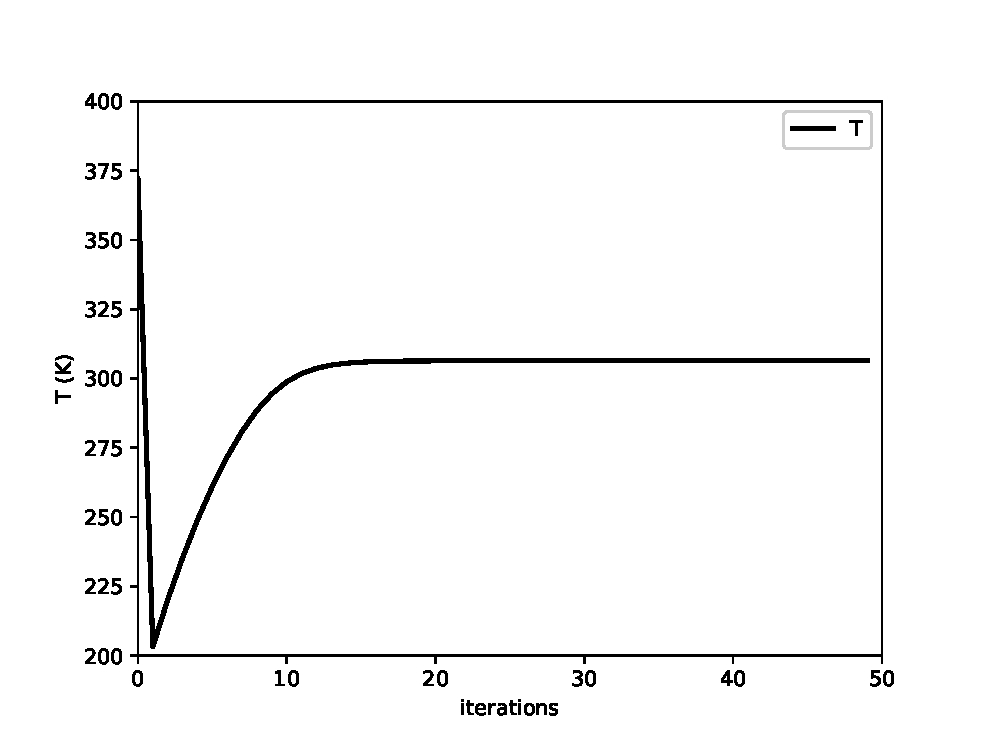
\includegraphics[scale=0.7]{DropletTIter.eps}
\caption{Iterative solution}
\label{fig:dropletTIter.eps}
\end{figure}

\end{document}
